\section{The New Empirical Industrial Organization}\label{sec:01-neio}

The cross-industry program of \cref{sec:01-scp} asked a single regression to separate demand, cost and conduct
across hundreds of industries. From the late 1970s the field moved in the opposite direction. Researchers studied
one industry at a time, wrote down an explicit model of its demand, cost and conduct, and estimated the conduct of
firms as a parameter. \citet{Bresnahan1989} named this program the \emph{New Empirical Industrial Organization}
(NEIO) and gave it its first systematic statement. This section presents the origins of the NEIO, its principles, its
workhorse model and its treatment of conduct. \Cref{sec:01-identification} then asks which features of the data
reveal market power. \Cref{fig:01-timeline} places the main contributions in time.

\begin{figure}[htbp]
\centering
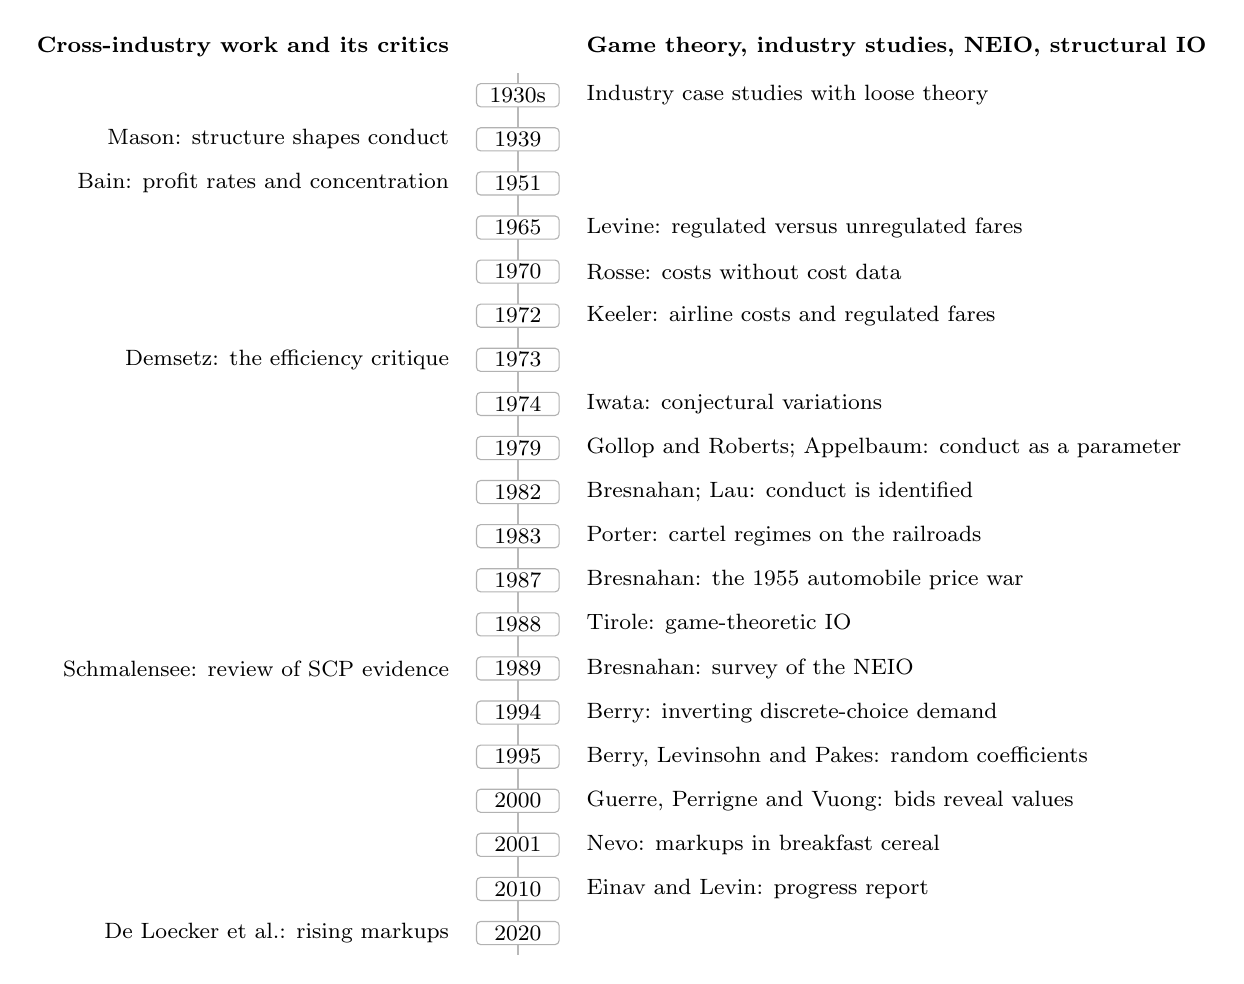
\begin{tikzpicture}[x=1cm, y=-0.56cm, every node/.style={font=\footnotesize}]
  \node[anchor=east, font=\footnotesize\bfseries] at (-0.75,-0.1) {Cross-industry work and its critics};
  \node[anchor=west, font=\footnotesize\bfseries] at (0.75,-0.1) {Game theory, industry studies, NEIO, structural IO};
  \draw[line width=0.8pt, gray!55] (0,0.5) -- (0,20.5);
  \foreach \y/\yr/\lt/\rt in {
    1/1930s//{Industry case studies with loose theory},
    2/1939/{Mason: structure shapes conduct}/,
    3/1951/{Bain: profit rates and concentration}/,
    4/1965//{Levine: regulated versus unregulated fares},
    5/1970//{Rosse: costs without cost data},
    6/1972//{Keeler: airline costs and regulated fares},
    7/1973/{Demsetz: the efficiency critique}/,
    8/1974//{Iwata: conjectural variations},
    9/1979//{Gollop and Roberts; Appelbaum: conduct as a parameter},
    10/1982//{Bresnahan; Lau: conduct is identified},
    11/1983//{Porter: cartel regimes on the railroads},
    12/1987//{Bresnahan: the 1955 automobile price war},
    13/1988//{Tirole: game-theoretic IO},
    14/1989/{Schmalensee: review of SCP evidence}/{Bresnahan: survey of the NEIO},
    15/1994//{Berry: inverting discrete-choice demand},
    16/1995//{Berry, Levinsohn and Pakes: random coefficients},
    17/2000//{Guerre, Perrigne and Vuong: bids reveal values},
    18/2001//{Nevo: markups in breakfast cereal},
    19/2010//{Einav and Levin: progress report},
    20/2020/{De Loecker et al.: rising markups}/%
  }{
    \node[fill=white, draw=gray!60, rounded corners=1.5pt, inner sep=1.6pt, minimum width=1.05cm] at (0,\y) {\yr};
    \node[anchor=east] at (-0.75,\y) {\lt};
    \node[anchor=west] at (0.75,\y) {\rt};
  }
\end{tikzpicture}
\caption[A timeline of empirical industrial organization]{A timeline of empirical industrial organization. Left:
the cross-industry tradition, its critics and its recent revival \citep{Mason1939,Bain1951,Demsetz1973,
Schmalensee1989,DeLoeckerEeckhoutUnger2020}. Right: game-theoretic IO, single-industry work, the NEIO and the
structural demand and supply models that followed \citep{Tirole1988,Levine1965,Rosse1970,Keeler1972,Iwata1974,
GollopRoberts1979,Appelbaum1979,Bresnahan1982,Lau1982,Porter1983,Bresnahan1987,Bresnahan1989,Berry1994,
BerryLevinsohnPakes1995,GuerrePerrigneVuong2000,Nevo2001,EinavLevin2010}. Rows are in chronological order and are
not drawn to scale.}
\label{fig:01-timeline}
\end{figure}

\subsection{Industry studies before the NEIO}\label{sec:01-early-studies}

Industry studies are older than the SCP paradigm. From the 1930s economists wrote detailed case studies of single
industries. These studies described pricing, capacity and rivalry with care. They made little attempt to generalize beyond the industry at hand, and the theory behind them was
loose. A case study could document that prices were high and stable. It could rarely say whether this reflected
market power, high costs or something else.

The clearest successes came in regulatory economics. \citet{Levine1965} compared air fares between Los Angeles
and San Francisco with fares in markets regulated by the Civil Aeronautics Board. Purely intrastate carriers on
this route, such as Pacific Southwest Airlines, were outside the Board's economic jurisdiction. The California
Public Utilities Commission, their only regulator, could not control entry in the period Levine studied
\citep[pp.~1430--1431]{Levine1965}. A state law signed on June 17, 1965, after Levine had written his article, gave the
Commission the power to regulate entry into intrastate air passenger service \citep[p.~1431, n.~63]{Levine1965}. The jet coach fare on this 350-mile route was about 3.9 cents per mile. The
national average jet coach fare was about 5.5 cents per mile, over longer stages that are cheaper to operate
\citep[p.~1433]{Levine1965}.
\citet{Keeler1972} estimated an airline cost function from interstate data and adjusted it to the operating
practices of the California intrastate carriers \citep[pp.~400--401]{Keeler1972}. He used seating densities
matching those of Pacific Southwest Airlines and a 60 percent load factor, below what the California carriers had
achieved \citep[pp.~405--406, 415 and 417]{Keeler1972}. The resulting
cost-based fares came within 3 percent of actual fares on two California intrastate routes. Among the 30 densest
routes in 1968, regulated coach fares exceeded these cost-based fares by 20 to 95 percent, and the markup tended
to rise with distance \citep[p.~416 and Table~6]{Keeler1972}. Both studies shaped the case for airline deregulation in the
late 1970s, the starting point of \cref{ch:airlines}. Their method compared prices with a competitive benchmark that
the data supplied directly, either an unregulated market or an estimate of cost.

\citet{Rosse1970} took a route that anticipated the NEIO. His title, which promises cost estimates ``without using cost
data'' (\cref{sec:01-lerner}), states the central idea of the later literature. He studied local newspapers, each treated as a
monopolist, and inferred marginal cost from the firm's pricing condition once demand had been estimated. The
application needed care because a newspaper sells two products. It sells circulation to readers and space to
advertisers, and the demand on each side depends on the other.

Let $Q^c$ denote circulation, $Q^a$ the column inches of advertising and $Q^e$ the column inches of editorial
content. The circulation price $P^c$ is the average price per subscription copy and the advertising price $P^a$ is
the average price per inch. Suppressing demand shifters and error terms, the inverse demands are
\begin{equation}\label{eq:01-rosse-demand}
P^a = P^a(Q^a, Q^c), \qquad P^c = P^c(Q^a, Q^c, Q^e).
\end{equation}
Advertisers pay more to reach more readers, so $\frac{\partial P^a}{\partial Q^c} > 0$. The newspaper chooses
$(Q^a, Q^c, Q^e)$ to maximize
\begin{equation*}
\Pi = P^a(Q^a, Q^c)\,Q^a + P^c(Q^a, Q^c, Q^e)\,Q^c - C(Q^a, Q^c, Q^e).
\end{equation*}
The marginal revenue of a product is the derivative of the firm's entire revenue with respect to that product's
quantity. For circulation, with $mc^c = \frac{\partial C}{\partial Q^c}$, the first-order condition is
\begin{equation*}
P^c + Q^c\frac{\partial P^c}{\partial Q^c} + Q^a\frac{\partial P^a}{\partial Q^c} - mc^c = 0 .
\end{equation*}
Solving for the circulation price gives the two-sided pricing condition \citep[eq.~6c]{Bresnahan1989}
\begin{equation}\label{eq:01-rosse-foc}
P^c = mc^c - Q^c\frac{\partial P^c}{\partial Q^c} - Q^a\frac{\partial P^a}{\partial Q^c} .
\end{equation}
The second term is the usual monopoly markup. The third term is new. It is the extra advertising revenue that one more
reader generates, and it lowers the circulation price. To see its size, divide \eqref{eq:01-rosse-foc} by $P^c$. Define
the inverse demand elasticities $f^c = -\frac{\partial \ln P^c}{\partial \ln Q^c} > 0$ and
$f^{ac} = \frac{\partial \ln P^a}{\partial \ln Q^c} > 0$. Then
\begin{align*}
\frac{P^c - mc^c}{P^c}
  &= -\frac{Q^c}{P^c}\frac{\partial P^c}{\partial Q^c} - \frac{Q^a}{P^c}\frac{\partial P^a}{\partial Q^c} \\
  &= f^c - \frac{P^a Q^a}{P^c Q^c}\cdot\frac{Q^c}{P^a}\frac{\partial P^a}{\partial Q^c}
   = f^c - \frac{P^a Q^a}{P^c Q^c}\, f^{ac} .
\end{align*}
The circulation price lies below marginal cost whenever $\frac{P^a Q^a}{P^c Q^c}\,f^{ac} > f^c$. This happens when
advertising revenue is large relative to circulation revenue and advertisers value readers highly. Most newspaper
revenue comes from advertising \citep[p.~1037]{Bresnahan1989}, so a reader price below marginal cost is a natural
outcome. A markup test applied to circulation alone would find price below marginal cost and could wrongly
conclude that newspapers have no market power. The theory of two-sided platforms later generalized this logic
\citep{RochetTirole2003,Armstrong2006}.

Rosse estimated the demand system \eqref{eq:01-rosse-demand} jointly with the pricing conditions. The
cross-equation restrictions between demand and marginal revenue then deliver marginal cost from the condition that
marginal cost equals marginal revenue. This let him treat marginal cost flexibly, for example by allowing transitory
shocks to firm size to separate short-run from long-run marginal cost. The approach is only as good as the estimated
marginal revenue. A linear demand curve may fit the data well and still give a poor estimate of its slope at the
observed point \citep[p.~1021]{Bresnahan1989}.

Two developments turned such isolated studies into a research program. The first was the critique of SCP regressions
developed in \cref{sec:01-scp-econometrics,sec:01-scp-after}. The second was the game theory revolution of the 1980s, which gave the field
sharp models of product differentiation, entry, pricing strategies and asymmetric information
\citep{Tirole1988}. Models proliferated so quickly that prominent members of the field lamented their overabundance
\citep{Fisher1989,Peltzman1991}. \citet[p.~146]{EinavLevin2010} note a lasting effect of this abundance. Because
predictions depended on fine details of preferences, information and commitment, empirical researchers learned to
take the institutional details of each market seriously. A single industry, studied with an explicit model, was the
natural place to do so.

\citet[Introduction]{Tirole1988} tells this history as two waves of interest in the field. The first was the
empirical Harvard tradition of \cref{sec:01-scp}. Alongside it, the ``Chicago tradition'' of Aaron Director and
George Stigler stressed rigorous theory and the empirical identification of competing theories. It also took a
permissive view of vertical restraints and predatory pricing, treating collusion as the main offense, and it
distrusted government intervention more than the Harvard tradition did. By the early 1970s many felt that theory
served more to explain statistical results or to buttress positions than to investigate markets systematically.
\citet[p.~273]{Joskow1975} wrote that ``the important messages are being carried by the informal theories,
stories, and behavioral observations.'' The formal models, in his phrase, were ``trotted out ex-post'' to show
that some formal apparatus could explain what was observed. Tirole attributes the second, mainly theoretical,
wave, which started in the 1970s, to three causes. On the demand side, researchers were dissatisfied with the
limits of cross-section work. On the supply side, leading theorists entered a field they had long ignored, and
noncooperative game theory became its standard tool. Game theory also made progress in two areas central to IO,
dynamics and asymmetric information. Tirole saw the new intra-industry studies of \citet{Porter1983} and
\citet{Bresnahan1987} as a sign that theory would soon feed back into empirical work (note~8).

\subsection{Principles of the NEIO}\label{sec:01-neio-principles}

\citet[p.~1012]{Bresnahan1989} summarizes the new approach in four ideas.
\begin{enumerate}
\item Price-cost margins are not observed. Economic marginal cost cannot be read from accounting data. The analyst
  infers it from firm behavior, uses differences between closely related markets to trace the effects of changes in
  marginal cost, or quantifies market power without measuring cost at all.
\item Industries have important idiosyncrasies. Institutional detail affects conduct, and it affects the measurement
  strategy even more. Comparative statics across industries are therefore suspect unless the markets are closely
  related.
\item Firm and industry conduct are unknown parameters. The behavioral equations by which firms set prices and
  quantities are estimated, and their parameters map into the notions of conduct of oligopoly theory.
\item The inference is explicit about its alternatives. The set of hypotheses is stated in advance. It includes the
  hypothesis of no strategic interaction, typically perfect competition, and the data can select it.
\end{enumerate}

The NEIO defined itself against three maintained hypotheses of the SCP paradigm \citep[pp.~1012--1013]{Bresnahan1989}.
The first was that economic price-cost margins can be observed in accounting data. The second was that
cross-industry differences in structure can be captured by a few observable measures, such as concentration ratios.
The third was that empirical work should estimate the reduced-form relation between structure and performance.
The gridlock over the meaning of high accounting profits, described in \cref{sec:01-demsetz}, showed where these
hypotheses led. No cross-industry regression could tell the market-power reading from the efficiency reading,
because both predict the same correlation.

The NEIO kept what the SCP paradigm had added to the field, namely systematic statistical evidence. It combined that
evidence with the attention to a single industry that marked the older case studies. In Bresnahan's words, the NEIO at
its best takes ``the best from the two great empirical IO traditions'' \citep[p.~1013]{Bresnahan1989}. A typical NEIO
paper is first of all an econometric model of one industry, with economic theory guiding both the specification and
the inference.

In practice these ideas translate into a recognizable research design.
\begin{itemize}
\item The unit of study is one industry, observed either as a time series or as a cross-section of geographic markets.
  Observations are similar to one another, so fewer factors are omitted than in a cross-section of industries.
\item Knowledge of the institutions guides the specification: which inputs matter, how the market clears, whether firms
  choose prices or quantities, and which prices are list prices and which are transaction prices.
\item Economic costs are inferred from pricing decisions rather than read from accounts. The inversion
  $\hat c = p\left(1 - \frac{1}{\hat\varepsilon^R}\right)$ of \cref{prop:01-infer-cost} is the simplest example.
\item Conduct is a parameter with an explicit interpretation (\cref{sec:01-conduct-parameter}).
\item External validity is claimed qualitatively. Some industries are studied as laboratories, for example ketchup,
  yogurt, laundry detergents or cement, and their value lies in mechanisms that travel to other markets. Others matter in
  their own right, for example health care, education, automobiles or airlines, and the specific numbers carry policy
  weight.
\end{itemize}
\citet[p.~147]{EinavLevin2010} make the same point about generality. The lasting lessons of industry studies tend to be
qualitative insights, such as the finding that entry can have large effects on prices, or methods that apply in many
settings.

A last principle concerns data. Economists in the field had long felt starved of appropriate data. The early NEIO
studies show this view to be false \citep[p.~1025]{Bresnahan1989}. The dissertations of Rosse, Bresnahan and Suslow
built their data from public industry sources, without relying on government statistics for the endogenous variables.
Porter's railroad data, discussed next, also came from industry records.

\subsection{Bresnahan's stylized model}\label{sec:01-stylized-model}

Most NEIO studies of homogeneous-good industries share one econometric structure. We present it in general form,
following \citet[Section~2.1]{Bresnahan1989} in the notation of this book, and then sketch Porter's study of a
railroad cartel as an illustration.

\casehead{Variables and equations}
Firms are indexed by $i = 1, \dots, N$ and observations, usually time periods, by $t$. The industry sells a single
product, so industry output $Q_t = \sum_i q_{it}$ is well defined. Demand has no intertemporal links from durability,
habits or learning. The endogenous variables are the market price $P_t$ and each firm's output $q_{it}$, or only
$Q_t$ when firm data are missing. Price-cost margins are not observed. The exogenous variables are demand shifters
$Y_t$, factor prices $W_{it}$ paid by firm $i$, and other cost shifters $Z_{it}$, such as fixed factors in a short-run
cost function. Three sets of unknown parameters describe demand ($\gamma$), cost ($\Gamma$) and conduct
($\vartheta$). The econometric errors $u^d_t$ and $u^c_{it}$ may enter nonlinearly and need not be scalars. The model
has five parts.
\begin{align}
P_t &= P(Q_t, Y_t, \gamma, u^d_t), \label{eq:01-bres-demand}\\
C_{it} &= C(q_{it}, W_{it}, Z_{it}, \Gamma, u^c_{it}), \label{eq:01-bres-cost}\\
mc_{it} &= C_q(q_{it}, W_{it}, Z_{it}, \Gamma, u^c_{it}), \label{eq:01-bres-mc}\\
P_t &= C_q(q_{it}, W_{it}, Z_{it}, \Gamma, u^c_{it}) - P_Q(Q_t, Y_t, \gamma, u^d_t)\, q_{it}\, \vartheta_{it}.
  \label{eq:01-bres-supply}
\end{align}
Equation \eqref{eq:01-bres-demand} is the inverse demand curve, \eqref{eq:01-bres-cost} the cost function and
\eqref{eq:01-bres-mc} marginal cost, where $C_q = \frac{\partial C}{\partial q}$. Equation \eqref{eq:01-bres-supply}
is the \emph{supply relation} of firm $i$, with $P_Q = \frac{\partial P}{\partial Q} < 0$ the slope of inverse
demand. Solving the demand equation and the $N$ supply relations together gives the reduced forms
\begin{equation}\label{eq:01-bres-rf}
P_t = P^*(W_t, Z_t, Y_t, \Theta, u_t), \qquad q_{it} = q_i^*(W_t, Z_t, Y_t, \Theta, u_t),
\end{equation}
where $\Theta = (\gamma, \Gamma, \vartheta)$ collects all parameters, $u_t$ all errors, and $W_t$ and $Z_t$ the
shifters of all firms. Equations \eqref{eq:01-bres-demand} to \eqref{eq:01-bres-rf} are Bresnahan's equations (1) to
(5) and (5$'$). We write $\Theta$ where Bresnahan writes $\Omega$, because $\Omega$ is the ownership matrix in this
book, and $\gamma$ where he writes $\delta$.

\casehead{The supply relation}
The supply relation states that marginal cost equals a ``perceived'' marginal revenue. For a monopolist,
$P + P_Q\,Q$ is marginal revenue. In \eqref{eq:01-bres-supply} the term $-P_Q\,q_{it}\vartheta_{it}$ is the wedge
between price and marginal cost, and $\vartheta_{it} \ge 0$ indexes how far the conduct of firm $i$ departs from price
taking. The value $\vartheta_{it} = 0$ is price taking. The value $\vartheta_{it} = 1$ is Cournot conduct and, with a
single firm, monopoly. Bresnahan calls it a supply relation because outside perfect competition firms have no
\emph{supply curve}, that is, no function $Q = S(P)$ that solves $P = mc(Q)$ \citep[fn.~6]{Bresnahan1989}. A firm
with market power chooses its output in response to the whole demand curve, including its slope, so the same price
can go with different outputs.

Equation \eqref{eq:01-bres-supply} seems to contain marginal cost, which the NEIO treats as unobserved. The
contradiction is only apparent. In the model, marginal cost is a function of the unknown parameters $\Gamma$, and it
can be computed only after $\Gamma$ has been estimated. Most methods estimate $\Gamma$ and $\vartheta$ in the same econometric step. A conduct parameter
that varies freely by firm and period would overparameterize the model. Bresnahan writes it this way only to nest all
known oligopoly theories, and every application restricts how $\vartheta_{it}$ varies.

\begin{remark}[Firm-level and industry conduct]\label{rem:01-firm-industry-conduct}
Bresnahan uses one symbol for two normalizations of conduct, and we keep them apart. The firm-level parameter
$\vartheta_{it}$ in \eqref{eq:01-bres-supply} equals $1 + r_i$ in the conjectural-variations notation of
\cref{sec:01-cournot-hhi}. It is $0$ for price taking, $1$ for Cournot and $N$ for symmetric collusion. The industry
parameter $\theta$ of this book weights each firm's conduct by its squared share, $\theta = \sum_i s_i^2\,\vartheta_i$,
as derived in \cref{prop:01-supply-relation} below. It is $0$ for price taking, $\HHI$ for Cournot and $1$ for collusion. With
symmetric firms, $q_{it} = \frac{Q_t}{N}$ and $s_i = \frac{1}{N}$, so
\begin{equation*}
\theta = \sum_{i=1}^{N} \frac{1}{N^2}\,\vartheta = \frac{\vartheta}{N}.
\end{equation*}
Symmetric Cournot ($\vartheta = 1$) gives $\theta = \frac{1}{N}$ and symmetric collusion ($\vartheta = N$) gives
$\theta = 1$, the convention used throughout the book.
\end{remark}

The core econometric methods are those for simultaneous equations, since $P_t$ and $q_{it}$ (or $Q_t$) are jointly
determined. Some studies estimate \eqref{eq:01-bres-demand} and \eqref{eq:01-bres-supply} directly as structural
equations, which is attractive because the conduct parameters are the object of interest. Studies that lack price,
quantity or firm-level data estimate reduced forms such as \eqref{eq:01-bres-rf} or aggregate the supply relations
to the industry level.

\subsubsection{An illustration: the Joint Executive Committee}\label{sec:01-porter-illustration}

\citet{Bresnahan1989} develops the stylized model alongside one application, Porter's (\citeyear{Porter1983}) study of
a nineteenth-century railroad cartel. We sketch that study here and draw out what it teaches about the NEIO. The full
case study, with the theory of \citet{GreenPorter1984} behind it and later reanalyses, appears in
\cref{ch:collusion-evidence}.

The Joint Executive Committee (JEC) was a legal cartel that controlled eastbound freight shipments from Chicago to the
Atlantic seaboard \citep[p.~302]{Porter1983}. Porter asks whether its prices switched between collusive and price-war
regimes, as trigger-price theories of collusion predict. The data are weekly records from the first week of 1880 to
the sixteenth week of 1886, which gives 328 observations. Quantity $Q_t$ is the tonnage of grain shipped by members,
and price $P_t$ is the grain rate in dollars per 100 pounds \citep[Table~2]{Porter1983}. Demand has constant
elasticity and shifts down when the Great Lakes are open to shipping. The supply relation is the industry version of
\eqref{eq:01-bres-supply}, derived in \cref{prop:01-supply-relation} below. Conduct takes a collusive value
$\theta^{c}$ in some weeks, and Porter normalizes conduct during price wars to the Bertrand value $\theta^{w} = 0$. He
treats each week's regime as an unobserved draw, collusive with a constant probability $\varpi$, and estimates the
system by maximum likelihood. We write $\varpi$ to keep $\pi$ for profit. Demand is inelastic, with an estimated
elasticity of $\hat\varepsilon = 0.80$ \citep[Table~3]{Porter1983}. With the lakes closed, predicted prices are 0.2780
dollars in collusive weeks and 0.1673 in price-war weeks \citep[Table~4]{Porter1983}. Collusion thus raised price by
66 percent and lowered quantity by 33 percent \citep[p.~310]{Porter1983}. The implied collusive conduct parameter is
$\hat\theta^{c} = 0.336$, which Porter calls roughly consistent with Cournot behavior \citep[p.~309]{Porter1983}.
\Cref{sec:13-jec} develops the model and estimates.

\citet[p.~1018]{Bresnahan1989} summarizes these findings in three statements. First, successful collusion raised
price by about 40 percent. This is the 0.40 reported for Porter in \cref{tab:01-bresnahan-table}. It measures the gap
from the collusive price, since $1 - \frac{0.1673}{0.2780} = 0.40$. Porter's 66 percent measures the same gap from
the price-war price. Second, the implied conduct was about as anticompetitive as Cournot. Only the gap between
the regimes is identified, because conduct during wars and the cost intercept enter the supply relation together. The
Cournot reading therefore rests on the unidentified assumption that price-war conduct was price taking (his
fn.~10). Third, the cartel broke down 28 percent of the time.

\casehead{What the illustration teaches}
Bresnahan sees three advantages in this structural approach \citep[p.~1018]{Bresnahan1989}. First, every parameter
has an economic meaning, so implausible estimates are diagnostic. Porter's demand elasticity is an example. With
$\hat\varepsilon = 0.80 < 1$, industry marginal revenue is negative, so the collusive weeks cannot reflect static joint
profit maximization \citep[p.~308]{Porter1983}. A conduct parameter of one would imply a Lerner index of
$\frac{1}{0.8} = 1.25$, which is impossible with positive marginal cost. Second, if the interpretation of conduct is
right, the link between the estimates and oligopoly theory is clear. Third, because the model is structural, the reason
why the data identify conduct can be stated. \Cref{sec:01-identification} takes up this third point.

Bresnahan also notes what the specification leaves out \citep[p.~1025]{Bresnahan1989}. A single constant probability
$\varpi$ tells us how often the cartel broke down. It cannot tell us what triggered breakdowns or what ended them,
which is where theories of collusion disagree. Answering that question needs a state-dependent switching probability.
Bresnahan doubts that the data can discriminate among the theories. A test of whether there are two regimes uses every
week of data, but a test of what starts and stops price wars has as many observations as there are price wars.

\subsection{Conduct as a parameter}\label{sec:01-conduct-parameter}

The stylized model treats conduct as an unknown parameter. This subsection derives the industry supply relation in
general form and lists the values of conduct implied by standard theories. It then surveys how the literature
specified conduct and explains how the estimates should and should not be read.

\begin{proposition}[Industry supply relation]\label{prop:01-supply-relation}
Consider a homogeneous good with differentiable inverse demand $P(Q)$, $P'(Q) < 0$, and $N$ firms with differentiable
costs $C_i(q_i)$. Firm $i$ chooses $q_i$ to maximize $P(Q)\,q_i - C_i(q_i)$, where $Q = q_i + Q_{-i}$ and the
conjectural variation $r_i = \frac{\dd Q_{-i}}{\dd q_i}$ of \cref{sec:01-cournot-hhi} is treated as a constant. Assume an interior solution
with every firm active, and let $mc_i = C_i'(q_i)$, $s_i = \frac{q_i}{Q}$ and $\varepsilon = -\frac{P}{Q\,P'(Q)}$.
Then:
\begin{enumerate}[label=(\roman*)]
\item Each firm satisfies the supply relation $P = mc_i - P'(Q)\,q_i\,(1 + r_i)$.
\item The industry satisfies
  \begin{equation}\label{eq:01-supply-relation}
  P = \overline{mc} - P'(Q)\,Q\,\theta, \qquad
  \overline{mc} = \sum_{i=1}^{N} s_i\, mc_i, \qquad
  \theta = \sum_{i=1}^{N} s_i^2 (1 + r_i).
  \end{equation}
\item Equivalently, $\frac{P - \overline{mc}}{P} = \frac{\theta}{\varepsilon}$, and average marginal cost can be
  recovered as $\overline{mc} = P + \theta\, Q\, P'(Q) = P\left(1 - \frac{\theta}{\varepsilon}\right)$.
\end{enumerate}
\end{proposition}

\begin{proof}
(i) The derivative of firm $i$'s profit is
\begin{equation*}
\frac{\dd}{\dd q_i}\Bigl[P(Q)\,q_i - C_i(q_i)\Bigr]
= P(Q) + q_i\,P'(Q)\,\frac{\dd Q}{\dd q_i} - C_i'(q_i)
= P + q_i\,P'(Q)\,(1 + r_i) - mc_i ,
\end{equation*}
because $\frac{\dd Q}{\dd q_i} = 1 + \frac{\dd Q_{-i}}{\dd q_i} = 1 + r_i$. Setting it to zero and solving for $P$
gives (i). (ii) Multiply (i) by $s_i$ and sum over $i$:
\begin{align*}
\sum_i s_i P &= \sum_i s_i\, mc_i - P'(Q)\sum_i s_i\, q_i (1 + r_i), \\
P &= \overline{mc} - P'(Q)\, Q \sum_i s_i^2 (1 + r_i),
\end{align*}
using $\sum_i s_i = 1$ and $q_i = s_i Q$. (iii) Subtract $\overline{mc}$ from both sides of \eqref{eq:01-supply-relation}
and divide by $P$:
\begin{equation*}
\frac{P - \overline{mc}}{P} = -\frac{Q\,P'(Q)}{P}\,\theta = \frac{\theta}{\varepsilon}.
\end{equation*}
Solving \eqref{eq:01-supply-relation} for $\overline{mc}$ gives the last statement.
\end{proof}

\Cref{prop:01-supply-relation} extends \cref{prop:01-clarke-davies} to marginal costs that vary with output. It shows
that one number, $\theta$, summarizes industry conduct for the purpose of the industry markup, whatever the
heterogeneity across firms. \Cref{tab:01-conduct-menu} lists the values implied by standard theories. The
inversion in part (iii) is the conduct-adjusted version of \cref{prop:01-infer-cost}. It is how the NEIO turns an
estimated demand curve and an assumed or estimated $\theta$ into an estimate of marginal cost.

\begin{table}[htbp]
\centering
\begin{threeparttable}
\caption{Conduct implied by standard oligopoly theories}
\label{tab:01-conduct-menu}
\small
\renewcommand{\arraystretch}{1.45}
\begin{tabular}{@{}lcccc@{}}
\toprule
Conduct & $r_i = \frac{\dd Q_{-i}}{\dd q_i}$ & $\vartheta_i = 1 + r_i$ & $\theta = \sum_i s_i^2(1 + r_i)$
  & $\frac{P - \overline{mc}}{P}$ \\
\midrule
Perfect competition & $-1$ & $0$ & $0$ & $0$ \\
Cournot & $0$ & $1$ & $\HHI$ & $\frac{\HHI}{\varepsilon}$ \\
Symmetric Cournot & $0$ & $1$ & $\frac{1}{N}$ & $\frac{1}{N\varepsilon}$ \\
Collusion (joint profit maximum) & $\frac{1 - s_i}{s_i}$ & $\frac{1}{s_i}$ & $1$ & $\frac{1}{\varepsilon}$ \\
Symmetric collusion & $N - 1$ & $N$ & $1$ & $\frac{1}{\varepsilon}$ \\
Clarke-Davies, $\kappa \in [0, 1]$ & $\kappa\frac{1 - s_i}{s_i}$ & $\frac{\kappa + (1 - \kappa)s_i}{s_i}$
  & $\kappa + (1 - \kappa)\HHI$ & $\frac{\kappa + (1 - \kappa)\HHI}{\varepsilon}$ \\
\bottomrule
\end{tabular}
\begin{tablenotes}\footnotesize
\item Notes: $s_i$ are output shares, $\HHI = \sum_i s_i^2$, and $\varepsilon$ is the market elasticity of demand.
Under collusion each firm acts as if rivals match its output in proportion to their shares, so
$1 + r_i = \frac{1}{s_i}$ and $\theta = \sum_i s_i = 1$. With constant marginal costs, the collusion rows require
equal costs across active firms. With rising marginal costs, they equalize marginal costs across firms. The
Clarke-Davies row is
\cref{prop:01-clarke-davies}: $s_i^2(1 + r_i) = (1 - \kappa)s_i^2 + \kappa s_i$, and summing gives
$\kappa + (1 - \kappa)\HHI$. Perfect competition requires rising marginal cost for an interior solution.
\end{tablenotes}
\end{threeparttable}
\end{table}

\subsubsection{How the literature specified conduct}\label{sec:01-conduct-taxonomy}

\citet[Section~2.2]{Bresnahan1989} sorts the early studies into four groups by how they wrote the supply relation. The
groups differ in language more than in substance.

\casehead{Supply relations from a single theory}
The first group derives $\vartheta_{it}$ from one explicit theory. The simplest case is monopoly or Cournot, where
$\vartheta_{it} = 1$ for all firms and periods \citep[eq.~6]{Bresnahan1989}:
\begin{equation*}
P_t = C_q(q_{it}, W_{it}, Z_{it}, \Gamma, u^c_{it}) - P_Q(Q_t, Y_t, \gamma, u^d_t)\,q_{it}.
\end{equation*}
With several firms this gives one estimating equation per firm. Rosse's newspapers, with the two-sided condition
\eqref{eq:01-rosse-foc}, belong here.

Bertrand pricing is the other static noncooperative model. With a homogeneous product and a flat marginal cost common to all firms
it is indistinguishable from perfect competition, so applications use differentiated products. \citet{Bresnahan1981}
estimates such a model on the 1977 and 1978 cross-sections of American automobiles. Products are ordered on a
one-dimensional quality index $\chi_j$, with neighbors $j - 1$ and $j + 1$. Consumers differ in a scalar taste for
quality. A consumer with taste $\nu$ who buys product $j$ at price $p_j$ gets $\nu\chi_j - p_j$, so she prefers $j$ to
$j + 1$ exactly when $\nu < \frac{p_{j+1} - p_j}{\chi_{j+1} - \chi_j}$. (Here $\nu$ is a taste for quality. Dividing
utility by $\nu$ gives the equivalent form with a consumer-specific price sensitivity used in \cref{ch:discrete}.) With
tastes spread uniformly with density $\gamma_0$, demand is
\begin{equation}\label{eq:01-vertical-demand}
q_j = \gamma_0\left(\frac{p_{j+1} - p_j}{\chi_{j+1} - \chi_j} - \frac{p_j - p_{j-1}}{\chi_j - \chi_{j-1}}\right) + u^d_j ,
\end{equation}
and quality is a hedonic function of observed characteristics $x_j$, such as length, weight and horsepower,
\begin{equation}\label{eq:01-vertical-quality}
\chi_j = f(x_j, \gamma_1) + u^{\chi}_j .
\end{equation}
These are Bresnahan's equations (7) and (8). Prices are manufacturer-to-dealer list prices, which equal transaction
prices for most sales, and quantities are model-year production. A firm $f$ owning the set of products
$\mathcal{J}_f$ chooses prices to maximize $\sum_{k \in \mathcal{J}_f} (p_k - mc_k)\,q_k$. Differentiating
\eqref{eq:01-vertical-demand},
\begin{equation*}
\frac{\partial q_j}{\partial p_j} = -\gamma_0\left(\frac{1}{\chi_{j+1} - \chi_j} + \frac{1}{\chi_j - \chi_{j-1}}\right),
\qquad
\frac{\partial q_{j+1}}{\partial p_j} = \frac{\gamma_0}{\chi_{j+1} - \chi_j},
\qquad
\frac{\partial q_{j-1}}{\partial p_j} = \frac{\gamma_0}{\chi_j - \chi_{j-1}} .
\end{equation*}
Let $\Omega_{jk} = 1$ if the same firm sells $j$ and $k$, and $\Omega_{jk} = 0$ otherwise. The matrix $\Omega$ is the
\emph{ownership matrix}, which returns in \cref{sec:01-workflow}. The first-order condition $q_j + \sum_{k \in \mathcal{J}_f}(p_k - mc_k)\frac{\partial q_k}{\partial p_j} = 0$ becomes
the supply relation
\begin{equation}\label{eq:01-vertical-foc}
q_j = \gamma_0 (p_j - mc_j)\left(\frac{1}{\chi_{j+1} - \chi_j} + \frac{1}{\chi_j - \chi_{j-1}}\right)
 - \Omega_{j,j+1}\,\gamma_0\,\frac{p_{j+1} - mc_{j+1}}{\chi_{j+1} - \chi_j}
 - \Omega_{j,j-1}\,\gamma_0\,\frac{p_{j-1} - mc_{j-1}}{\chi_j - \chi_{j-1}} ,
\end{equation}
the counterpart of Bresnahan's equation (6$''$). Marginal cost depends on the characteristics of the product. The
markup of product $j$ is large when its neighbors are far away in quality space. \citet{Bresnahan1981} finds large
price-cost margins on the larger cars, which are also much farther apart in quality space. The obvious weakness is the
restrictive demand system. Bresnahan probes it through the residuals, firm dummies and the quality error in
\eqref{eq:01-vertical-quality}. \Cref{ch:discrete} develops the vertical model in full.

A second class of single theories gives firms different roles. In the \emph{Stackelberg} model, firms
$2, \dots, N$ follow Cournot supply relations and the leader, firm 1, internalizes their reaction. Its supply relation is
\begin{equation}\label{eq:01-stackelberg}
P_t = C_q(q_{1t}, W_{1t}, Z_{1t}, \Gamma, u^c_{1t}) - P_Q(Q_t, Y_t, \gamma, u^d_t)\,q_{1t}\,(1 + \theta_S),
\end{equation}
where $\theta_S$ is the derivative of the followers' total output with respect to $q_1$, obtained by solving their
supply relations. A linear example shows what $\theta_S$ looks like. Let $P = a - bQ$ and let the $N - 1$ followers
have constant marginal cost $c$. Follower $j$'s Cournot condition is $a - bQ - b q_j = c$. Summing over the followers,
with $Q = q_1 + Q_F$ and $Q_F$ their total output,
\begin{align*}
(N - 1)(a - c) - (N - 1)\,b\,(q_1 + Q_F) - b\,Q_F &= 0, \\
Q_F &= \frac{(N - 1)(a - c - b\,q_1)}{N b}.
\end{align*}
Hence $\theta_S = \frac{\dd Q_F}{\dd q_1} = -\frac{N - 1}{N}$, and the leader's firm-level conduct is
$\vartheta_1 = 1 + \theta_S = \frac{1}{N}$. The leader behaves more aggressively than a Cournot firm because each unit
it adds displaces part of the followers' output.

The \emph{dominant-firm} model is closely related. \citet{Suslow1986} estimates it for Alcoa in the interwar period,
when Alcoa was the only producer of new aluminum and a fringe of firms recycled scrap. The fringe takes price as given,
so its supply relation is a supply curve. Write it as $Q_{ft} = S(P_t, W_{ft}, Z_{ft}, \Gamma, u^c_{ft})$, the inverse
of $P_t = C_q(Q_{ft}, \dots)$. Bresnahan's equations (10) and (10$'$) are these two forms. The dominant firm faces the
residual demand $q_1 = Q(P) - S(P)$, where $Q(P)$ is market demand. Its slope is
\begin{equation*}
\frac{\dd P}{\dd q_1} = \frac{1}{Q'(P) - S_P} = \frac{P_Q}{1 - P_Q S_P},
\end{equation*}
where $P_Q = \frac{1}{Q'(P)} < 0$ and $S_P = \frac{\partial S}{\partial P} \ge 0$. The first-order condition
$P + q_1\frac{\dd P}{\dd q_1} = mc_1$ can be written in the form of \eqref{eq:01-bres-supply}:
\begin{equation}\label{eq:01-dominant}
P_t = mc_{1t} - P_Q\,q_{1t}\,(1 + S_D), \qquad S_D = \frac{P_Q S_P}{1 - P_Q S_P} \in (-1, 0].
\end{equation}
These are Bresnahan's equations (11) and (11$'$). With no fringe response ($S_P = 0$) the leader is a monopolist on its residual demand and $S_D = 0$. As the fringe supply becomes
perfectly elastic, $S_D \to -1$ and the leader becomes a price taker. In elasticity form, with $s_1$ the leader's share
and $e_S$ the fringe supply elasticity, $P_Q S_P = -\frac{(1 - s_1)e_S}{\varepsilon}$, and
\begin{equation*}
\frac{P - mc_1}{P} = \frac{s_1}{\varepsilon}\,(1 + S_D) = \frac{s_1}{\varepsilon + (1 - s_1)\,e_S} .
\end{equation*}
In Suslow's data Alcoa's marginal cost is shifted by its accounting average variable cost, which does not enter the fringe
supply. The fringe supply is shifted by the stock of aluminum available for recycling. She estimates $S_D$ to be small, so
Alcoa had considerable market power despite the fringe \citep[p.~1023]{Bresnahan1989}. She identifies Alcoa as the
leader from the structure of the industry, a monopoly in new aluminum facing many recyclers.

Dynamic theories of collusion form the last part of this group. \citet{Stigler1964} argued that cartels held together
by self-interest should sometimes break down. Firms cannot always tell whether a fall in their sales reflects secret
price cutting, so suspicion leads to price wars even without cheating. \citet{GreenPorter1984} formalized this idea.
Firms observe the market price but not rivals' outputs, and a low price triggers a reversion to Cournot behavior for a
fixed period. The cartel chooses the collusive output, the trigger price and the length of punishment to maximize
expected profit. It does not push price to the monopoly level, because a higher price raises the gain from cheating.
\citet{AbreuPearceStacchetti1986} find more profitable designs in which both the start and the end of a price war are
triggered, so wars have random length and endogenous severity. \citet{RotembergSaloner1986} let demand fluctuate. When
current demand does not predict future demand, the gain from defecting is largest in booms, so the cartel must lower
its price in booms. All these theories imply that $\vartheta_{it}$ varies over time. They differ in the predicted
timing of the regimes, which is why Porter's constant $\varpi$ cannot tell them apart. \Cref{ch:collusion-theory}
develops these models.

\casehead{Testing a small set of theories}
A second group estimates the supply relations of a few distinct theories and tests among them.
\citet{Bresnahan1987} uses the vertical model \eqref{eq:01-vertical-demand} for the American automobile industry in
the mid-1950s. Under joint profit maximization, $\Omega_{jk} = 1$ for every pair of neighbors in
\eqref{eq:01-vertical-foc}, because industry marginal revenue counts every product. Under Bertrand pricing $\Omega_{jk}$
follows actual ownership.
Non-nested tests favor collusion in 1954 and 1956 and Bertrand competition in 1955, the year of a large expansion of
output and a fall in prices. A temporary breakdown of collusion thus explains part of the 1955 boom. \Cref{ch:discrete}
treats this paper as a case study. \citet{Geroski1983} and \citet{Roberts1984} test leader-follower theories on the
coffee-roasting data of \citet{GollopRoberts1979}. The smaller roasters behave as price-taking followers. The leading
firms behave less competitively than Cournot firms. They stop short of maximizing joint profits, even given the
fringe \citep[p.~1026]{Bresnahan1989}.

The difference between estimating a continuous $\vartheta$ and choosing among a few theories is purely econometric
\citep[p.~1026]{Bresnahan1989}. A researcher who estimates $\vartheta$ on a continuum tests theories with nested tests,
and may find a value between two theories. A researcher who specifies a few theories uses non-nested tests.

\casehead{Conjectural-variations language}
A third group writes conduct as a conjectural variation, a firm's ``expectation'' of how rivals' outputs respond
to its own. Starting with \citet{Iwata1974}, these papers write the supply relation as
\begin{equation}\label{eq:01-cv-supply}
P_t = C_q(\cdot) - P_Q(\cdot)\, q_{it}\,\bigl(1 + r_i(q_{it}, Q_{-i,t}, Z_{it}, \Phi)\bigr),
\end{equation}
where the parameters $\Phi$ let conjectures depend on firm size and other variables. Iwata asked where the Japanese
plate glass industry lay between competition and monopoly. He assumed, unlike most later work, that accounting data
reveal margins. \citet{GollopRoberts1979} let conjectures differ across firms in coffee roasting, and
\citet{SpillerFavaro1984} and \citet{GelfandSpiller1987} continued this emphasis on heterogeneous conduct in banking.

Equation \eqref{eq:01-cv-supply} differs from \eqref{eq:01-bres-supply} only in replacing $\vartheta_{it}$ by
$1 + r_i(\cdot)$. As a matter of logic the two are identical, since $\vartheta_{it} - 1 = r_i(\cdot)$ nests the same
models. Bresnahan puts it strongly: saying what the conjectural variation is and saying which theory of oligopoly holds
in the data are the same statement \citep[p.~1027]{Bresnahan1989}. The practical differences are two.
Conjectural-variation papers allow all values of $r_i$, and they stress the link between firm size and conduct.

\casehead{Aggregate data and average conduct}
A fourth group has only industry data. It writes the supply relation in aggregate form \citep[eq.~16]{Bresnahan1989},
\begin{equation}\label{eq:01-aggregate-supply}
P_t = C_q(Q_t, W_t, Z_t, \Gamma, u^c_t) - P_Q(Q_t, Y_t, \gamma, u^d_t)\, Q_t\, \theta_t ,
\end{equation}
as in \citet{Appelbaum1979} and Porter's study. Under the null of price taking ($\theta_t = 0$), $C_q$ is industry
marginal cost. With market power, firms generally have different marginal costs in equilibrium. Cournot firms with
different costs have different margins \citep{CowlingWaterson1976}, so a stable industry marginal cost curve need not
exist. \Cref{prop:01-supply-relation} gives the right reading. The aggregate $\theta_t = \sum_i s_{it}^2\vartheta_{it}$
weights each firm's conduct by its squared share, and $\frac{P - C_q}{P}$ is the share-weighted average markup. Some authors claimed that oligopoly theory implies identical
conduct across firms \citep{Appelbaum1982,Lopez1984}. Bresnahan rejects this claim, since nothing in oligopoly theory
forces firms to behave alike.

\subsubsection{What an estimated conjecture means}\label{sec:01-cv-warning}

The language of conjectures invites a misreading \citep[pp.~1027--1029]{Bresnahan1989}. Suppose we read
\eqref{eq:01-cv-supply} as the first-order condition of a firm that expects rivals' outputs to depend on its own:
\begin{equation}\label{eq:01-cv-profit}
\max_{q_i}\; P\Bigl(q_i + \sum_{j \ne i} Q_j(q_i)\Bigr)\, q_i - C(q_i),
\qquad
1 + r_i = \frac{\dd q_i}{\dd q_i} + \sum_{j \ne i} \frac{\dd Q_j}{\dd q_i} .
\end{equation}
For Cournot conduct ($r_i = 0$) and price taking ($r_i = -1$) the reading is harmless. A Cournot firm can be described as
expecting rivals' outputs to stay fixed, and a competitive firm as expecting price to stay fixed.

The trouble arises near collusion. Let all $N$ firms have the same costs and the collusive conjecture $1 + r_i = N$.
Each supply relation becomes
\begin{equation}\label{eq:01-collusive-foc}
P = C_q(\cdot) - P_Q(\cdot)\, N\, q_i ,
\end{equation}
which is the first-order condition for maximizing the joint profit of all $N$ firms. Read literally, $r_i = N - 1$ says
that each firm expects every rival to match any change in its output one for one, $\frac{\dd Q_j}{\dd q_i} = 1$. Repeated
games give a different account of the same outcome. Firms produce their share of the collusive output because they expect
a deviation to trigger a general breakdown of restraint. The matching behavior is never observed. It is the threat that
keeps it off the equilibrium path.

Bresnahan therefore separates two objects: (i) what firms believe will happen if they deviate, and (ii) what firms do
as a result of those beliefs. Estimated conjectures measure only (ii). If they are stable over time and breakdowns are
rare, they measure the average collusiveness of conduct. They carry no information about what would happen if one
firm expanded output on its own, which is the sense of ``conjectural variation'' in theoretical work. The only thing
they reveal about expectations is that the expectations suffice to deter departures from the normal arrangement
\citep[fn.~19]{Bresnahan1989}. For the same reason Bresnahan rejects reading the slope of $r_i(\cdot)$ in own output as
evidence of ``mutual forbearance''.

A second interpretive issue concerns firm size. Models with different conjectures for different size classes produce
an equilibrium size distribution even among identical firms. A competing explanation is that firms differ in cost.
Separating the two requires firm-specific cost functions, and in particular a comparison of the marginal costs of large
and small firms at the same output \citep[p.~1030 and fn.~20]{Bresnahan1989}.

\subsubsection{Every specification is a test of price taking}\label{sec:01-appelbaum}

\citet{Appelbaum1979} observed that setting every conduct parameter to zero in \eqref{eq:01-bres-supply}, or every
$r_i$ to $-1$, imposes price taking. Every specification of conduct, theoretical or not, therefore nests the
competitive model. Its estimation is a test of price-taking behavior, the title of Appelbaum's paper, against an
alternative in which firms raise price above marginal cost. This is the advance that the NEIO claims over the SCP
paradigm \citep[p.~1031]{Bresnahan1989}. When price taking is rejected, it is rejected against specific theories of
market power. The interpretation of the result is then clear, and only econometric problems can cloud the inference.

Two cautions carry over to later chapters. First, an estimated $\theta$ is a reduced summary of behavior, as the
discussion of conjectures shows. \citet{Corts1999} shows that when firms collude dynamically, the estimated $\theta$
tracks how the markup responds to demand shocks at the margin. It can then differ greatly from the average markup that
it is meant to measure. His Proposition~1 (p.~233) states the condition exactly, for linear demand, constant
marginal cost and a symmetric equilibrium. Let $q^*$ be equilibrium output per firm and $Y$ a demand shifter. The
estimate equals the elasticity-adjusted Lerner index that $\theta$ is meant to measure if and only if
\[
\frac{P - mc}{q^*} = \frac{\frac{\dd (P - mc)}{\dd Y}}{\frac{\dd q^*}{\dd Y}} .
\]
The margin per unit of output must equal the marginal response of the margin to output along demand-driven
movements. Under efficient supergame collusion this condition fails. The estimated conduct parameter then
understates market power unless demand shocks are fully permanent. When the shocks are completely transitory, it
may detect no market power at all, even if average margins are near the monopoly level (p.~245).
\Cref{ch:conduct} develops this critique. Second, the theory of the conduct parameter, including
its links to conjectural variations and pass-through, appears in \cref{ch:theory}.

\section{How the data identify market power}\label{sec:01-identification}

A structural model states the class of hypotheses among which the data choose. This makes a central question
answerable \citep[p.~1031]{Bresnahan1989}. Why do the data identify the inference of market power? Which implication
of perfect competition has been rejected when market power is measured? The question does not arise in the SCP
paradigm, which takes margins to be observed. In the NEIO margins are estimated, so we must ask which features of the
data and which natural experiments reveal them. Bresnahan distinguishes four classes of arguments: comparative statics
in demand, comparative statics in cost, direct estimation of marginal cost, and supply shocks. A fifth, comparative
statics in industry structure, is familiar in its logic but still lacked a sound identification argument in 1989. This
section explains each, then turns to differentiated products and to what the NEIO learned.

\subsection{The identification question}\label{sec:01-id-question}

The question is this. Given equilibrium prices and quantities from different but similar markets, under what conditions
can we identify conduct, or test for market power, without observing demand and cost? A linear model shows the
difficulty. Let demand and marginal cost be
\begin{equation}\label{eq:01-linear-id-model}
Q_t = a_0 + a_1 P_t + a_2 Y_t + u^d_t, \qquad mc_t = b_0 + b_1 Q_t + b_2 W_t + u^c_t ,
\end{equation}
with $a_1 < 0$, a demand shifter $Y_t$ and a cost shifter $W_t$. The slope of inverse demand is $\frac{1}{a_1}$, so the
supply relation of \cref{prop:01-supply-relation} is $P_t = mc_t - \theta\frac{Q_t}{a_1}$. Substituting marginal cost,
\begin{equation}\label{eq:01-linear-supply}
P_t = b_0 + \left(b_1 - \frac{\theta}{a_1}\right) Q_t + b_2 W_t + u^c_t .
\end{equation}
The cost shifter $W_t$ is excluded from demand, so it identifies $(a_0, a_1, a_2)$. The demand shifter $Y_t$ is
excluded from the supply relation, so it identifies $b_0$, $b_2$ and the slope $b_1 - \frac{\theta}{a_1}$. The two
parameters $b_1$ and $\theta$ enter only through this slope. A competitive industry with steep marginal cost and a
monopoly with flatter marginal cost produce the same data. When demand shifts out, price rises in both, either because
marginal cost rises with output or because of market power. Demand shifts that move the curve in parallel cannot tell
the two apart. \Cref{ch:conduct} develops this observational equivalence in detail, with figures, and shows how
\citet{Bresnahan1982} breaks it. The next subsection previews the general arguments.

\subsection{Five identification arguments}\label{sec:01-id-arguments}

\subsubsection{Comparative statics in demand}\label{sec:01-id-demand}

The first argument, due to \citet{Bresnahan1982} and \citet{Lau1982}, uses demand shifters that change the slope of
demand. \citet[Section~3.1]{Bresnahan1989} presents it in a simple version. Errors are additive, conduct $\theta$ is
constant, and the slope of inverse demand depends on the demand shifters but not on quantity. The demand equation and
the aggregate supply relation \eqref{eq:01-aggregate-supply} become
\begin{align}
P_t &= P(Q_t, Y_t, \gamma) + u^d_t, \label{eq:01-id-demand}\\
P_t &= C_q(Q_t, W_t, Z_t, \Gamma) + u^c_t - P_Q(Y_t, \gamma)\, Q_t\, \theta . \label{eq:01-id-supply}
\end{align}
Demand \eqref{eq:01-id-demand} has one endogenous regressor, $Q_t$, and the cost shifters provide instruments, so
$\gamma$ can be estimated. Call the estimate $\hat\gamma$ and form the constructed variable
$\hat P_{Q,t} = P_Q(Y_t, \hat\gamma)$. Then consider
\begin{equation}\label{eq:01-id-twostep}
P_t = C_q(Q_t, W_t, Z_t, \Gamma) + u^c_t - \hat P_{Q,t}\, Q_t\, \theta .
\end{equation}
Equations \eqref{eq:01-id-demand} to \eqref{eq:01-id-twostep} are Bresnahan's (17) to (19). Bresnahan calls the
two-step procedure too ugly for anyone to use, but it shows why better estimators identify $\theta$.

Equation \eqref{eq:01-id-twostep} has two endogenous variables: $Q_t$, which enters cost, and $\hat P_{Q,t}Q_t$, whose
coefficient is $\theta$. Two conditions are needed to estimate $\theta$. First, the two variables must not be
perfectly collinear. If the slope of demand does not depend on $Y_t$, then $\hat P_{Q,t}$ is a constant and
$\hat P_{Q,t}Q_t$ is proportional to $Q_t$. This is exactly the linear model above. Second, there must be instruments
for both endogenous variables. Both conditions hold when $Y_t$ has two elements, one that enters the slope $P_Q$ and one
that does not. A linear example is the inverse demand
\begin{equation*}
P_t = \gamma_0 + \gamma_1 Y_{1t} + (\gamma_2 + \gamma_3 Y_{2t})\, Q_t + u^d_t ,
\end{equation*}
in which $Y_{1t}$ shifts demand and $Y_{2t}$ rotates it. \citet{Lau1982} gives a general sufficient condition. The
parameter $\theta$ is identified if the inverse demand function cannot be written as $P(Q, Y) = \tilde P(Q, h(Y))$ for
a scalar index $h$. With a single demand shifter the index form holds trivially, with $h(Y) = Y$, so
identification requires at least two demand shifters.

\begin{remark}[Why a single demand index is not enough]\label{rem:01-lau}
Suppose $P(Q, Y) = \tilde P(Q, h(Y))$ with scalar $h$, and ignore errors. Fix $W$ and let $Q^*(h, W)$ be the
equilibrium quantity of a model with conduct $\theta > 0$ and marginal cost $C_q(Q, W)$. Assume $Q^*$ is strictly
monotone in $h$, with inverse $h = H(Q, W)$. Define a new marginal cost $mc^{\dagger}(Q, W) = \tilde P(Q, H(Q, W))$,
which depends only on cost variables. Consider a competitive industry with this marginal cost, and assume its
equilibrium is unique. For any $(h, W)$, the quantity $Q^*(h, W)$ satisfies $\tilde P(Q, h) = mc^{\dagger}(Q, W)$
because $H(Q^*(h, W), W) = h$. The competitive
model therefore reproduces every equilibrium of the model with market power, and $\theta$ is not identified without
restrictions on cost. With two demand shifters this construction fails. Two values of $Y$ can produce the same
equilibrium quantity with different slopes of demand. Competition then predicts the same price for both, while market
power predicts different prices.
\end{remark}

The economics is simple \citep[p.~1033]{Bresnahan1989}. Suppose the demand shifters could rotate the demand curve
around the equilibrium point. Under perfect competition nothing happens, because supply and demand still cross at the
same point. Under monopoly or any oligopoly theory, the change in the elasticity of demand shifts perceived marginal
revenue, and price and quantity respond. Market power has an idiosyncratic comparative static, and the data can detect
it.

Applications need a natural experiment that changes the slope of demand. In \citet{JustChern1980} the market power lies
on the buying side. A concentrated processing industry buys tomatoes from many farmers, and the adoption of a
mechanical harvester changed the elasticity of supply. The logic is the same as for sellers. In
\citet{Bresnahan1981,Bresnahan1987} elasticities depend on how close products are in quality space. More generally,
one shifter might measure the size of the economy, such as national income, and a second the price of a substitute.
The method stands or falls with the estimated demand elasticities. Critics offered other readings of the tomato
harvester, and the automobile results depend on the ordering of products in quality space.

A second route uses the structure of cost. Suppose marginal cost is homogeneous of degree one in factor prices, as it is
whenever it is derived from a cost function. Then every term of marginal cost involves a factor price. Any term in the
supply relation that does not involve a factor price must belong to the markup \citep[p.~1034]{Bresnahan1989}. For example, if
$C_q(Q, W) = \sum_k W_k\, g_k(Q)$, the supply relation
\begin{equation*}
P_t = \sum_k W_{kt}\, g_k(Q_t) - \theta\, Q_t\, P_Q(Q_t, Y_t, \gamma) + u^c_t
\end{equation*}
identifies $\theta$ from the one term that no factor price multiplies. This is how \citet{Appelbaum1979,Appelbaum1982}
obtained identification. The argument leans heavily on the functional form of marginal cost and on observing the true
marginal price of every input, capital in particular. The defense is robustness to other functional forms, to
quasi-fixed capital and labor, and to economic rather than accounting costs of capital. \Cref{ch:conduct} gives the
full treatment of identification through demand, with figures and estimation.

\subsubsection{Comparative statics in cost}\label{sec:01-id-cost}

\citet{PanzarRosse1987} propose two ideas. The first is to estimate a reduced form and to focus on the coefficients of
factor prices. The second is that a reduced-form revenue equation can be estimated even where price and quantity are
not observed. Let firm $i$'s equilibrium revenue be
\begin{equation}\label{eq:01-pr-revenue}
R_{it} = R^*(W_{it}, Z_{it}, Y_t, \Theta, u_t),
\end{equation}
obtained by solving demand and the supply relations for price and quantity and multiplying them. The
\emph{Panzar-Rosse statistic} is the sum of the elasticities of reduced-form revenue with respect to all factor prices,
\begin{equation}\label{eq:01-pr-stat}
\psi = \sum_k \frac{\partial R^*}{\partial W_k}\,\frac{W_k}{R^*} .
\end{equation}
Equations \eqref{eq:01-pr-revenue} and \eqref{eq:01-pr-stat} are Bresnahan's (20) and (21), where the statistic is
called $H_R$. It needs little data on endogenous variables, but it needs every variable that shifts cost or demand.
Revenue also avoids a quality correction. If the product is better in some markets, price per unit overstates the true
price there, but revenue is unaffected.

For an elementary monopolist, which chooses one quantity, $\psi$ has a definite sign. Let $R(Q, Y) = Q\,P(Q, Y)$ be
revenue as a function of output, so that $R_Q$ is marginal revenue. Let $Q^*(W)$ solve $R_Q(Q) = C_Q(Q, W)$, and let
equilibrium revenue be $R^*(W) = R(Q^*(W))$. Differentiating the first-order condition with respect to $W_k$,
\begin{equation*}
R_{QQ}\,\frac{\partial Q^*}{\partial W_k} = C_{QQ}\,\frac{\partial Q^*}{\partial W_k} + C_{QW_k}
\quad\Longrightarrow\quad
\frac{\partial Q^*}{\partial W_k} = \frac{C_{QW_k}}{R_{QQ} - C_{QQ}} .
\end{equation*}
Then $\frac{\partial R^*}{\partial W_k} = R_Q \frac{\partial Q^*}{\partial W_k}$. Because $C$ is homogeneous of degree
one in $W$, so is $C_Q$, and Euler's theorem gives $\sum_k W_k C_{QW_k} = C_Q$. At the optimum $C_Q = R_Q$. Hence
\begin{equation}\label{eq:01-pr-monopoly}
\psi = \frac{1}{R^*}\sum_k W_k\,R_Q\,\frac{C_{QW_k}}{R_{QQ} - C_{QQ}}
     = \frac{R_Q\,C_Q}{(R_{QQ} - C_{QQ})\,R^*}
     = \frac{(R_Q)^2}{(R_{QQ} - C_{QQ})\,R^*} \le 0 ,
\end{equation}
since the second-order condition requires $R_{QQ} - C_{QQ} < 0$. This is Bresnahan's equation (23). The intuition is
direct. A one percent increase in all factor prices raises marginal cost by one percent, and a monopolist's revenue
always falls when its costs rise. Otherwise its output was too large before the increase. \citet{PanzarRosse1987} show
that the result holds for a monopolist with many choice variables, including several outputs, quality or advertising.

A second hypothesis also has a sharp prediction. In long-run competitive equilibrium with free entry, every firm
produces at the minimum of its average cost. A proportional increase in all factor prices raises minimum average cost in
the same proportion and leaves the efficient scale unchanged. Firm revenue, the product of the two, rises in the same
proportion, so $\psi = 1$. Industry output falls through exit. In this case demand shifters should not enter the
revenue equation, which gives a second testable restriction \citep[p.~1037 and fn.~30]{Bresnahan1989}.

The statistic does not discriminate perfectly. It need not be positive when firms are not monopolists, although
\citet{PanzarRosse1987} show that it is positive in some models of oligopoly and monopolistic competition. A negative
$\psi$ can also arise for reasons other than monopoly, so false findings of monopoly are possible. The applications
use cross-sections of similar local markets. \citet{PanzarRosse1977} study newspapers in local media markets and reject
monopoly even for newspapers that are alone in their market, which points to competition from other media.
\citet{Shaffer1982} studies banks in New York State in 1979 and rejects both monopoly and long-run competition. These
studies are convincing to the extent that the cross-section reflects long-run equilibria and every cost shifter is
measured and correctly entered. \Cref{ch:conduct} proves the results above and discusses the test further.

A per-unit tax is the cleanest cost shifter, because it enters marginal cost one for one and is observed.
\citet{Sumner1981} builds a test of monopoly pricing on state cigarette excise taxes. Let a firm face a residual
demand elasticity $\varepsilon^R > 1$ that is constant over the sample. Its marginal cost is $mc = X\phi + E + R$,
where $X$ contains observed cost factors, $E$ unobserved ones and $R$ the tax per pack. Marginal revenue equals
marginal cost when
\[
P = \frac{\varepsilon^R}{\varepsilon^R - 1}\, mc
\]
(his equations 1 and 2, with his elasticity $\eta = -\varepsilon^R$). Multiplying out and absorbing the factor
$\frac{\varepsilon^R}{\varepsilon^R - 1}$ into the coefficients of $X$ gives his estimating equation (4), for
state $i$ in year $t$,
\begin{equation}\label{eq:01-sumner}
P_{it} = X_{it}\phi + \rho R_{it} + U_{it}, \qquad \rho = \frac{\varepsilon^R}{\varepsilon^R - 1} = \frac{P}{mc} .
\end{equation}
Sumner calls the tax coefficient $\theta$. We write $\rho$ because the coefficient is a pass-through rate that
equals the ratio of price to marginal cost. It differs from the conduct parameter $\theta$ of
\cref{sec:01-conduct-parameter}. Competition with constant marginal cost implies $\rho = 1$. The data
are 1,200 state-years, for 47 states and the District of Columbia over 1954--1978, and the estimator is OLS. With
state and year dummies in $X_{it}$, $\hat\rho = 1.074$ (0.013). With the national consumer price index in place of
the dummies, $\hat\rho = 1.029$ (0.011), and a variance-components model gives $1.069$ (0.013) (Table~1,
p.~1017). Sumner reports implied firm elasticities of 13.5, 34.5 and 14.5 in absolute value. Every estimate is
significantly above one, so atomistic competition is rejected. Yet the firm elasticities lie far above the
industry elasticities of 0.3 to 0.8 found in other studies (p.~1017), so an effective cartel is rejected too.
The reported elasticities equal $\frac{1}{\hat\rho - 1}$, and \cref{ch:conduct} compares them with the exact
inversion of \eqref{eq:01-sumner} in its full treatment of the paper.

\citet{Sullivan1985} and \citet{AshenfelterSullivan1987} extend the idea to settings where market price and quantity
are observed. Let all firms share a constant marginal cost $c$, and let firm $i$ satisfy the supply relation
$P = c - P'(Q)\,q_i\,(1 + r_i)$. Solving for output and summing over firms,
\begin{equation*}
q_i = \frac{P - c}{-P'(Q)\,(1 + r_i)}
\quad\Longrightarrow\quad
Q = \frac{P - c}{-P'(Q)}\sum_i \frac{1}{1 + r_i}
  = (P - c)\,\frac{\varepsilon\, Q}{P}\sum_i \frac{1}{1 + r_i},
\end{equation*}
using $-\frac{1}{P'(Q)} = \frac{\varepsilon Q}{P}$. Dividing by $Q$ gives $\sum_i (1 + r_i)^{-1} = \frac{1}{\varepsilon L}$,
where $L = \frac{P - c}{P}$. Now let $E_P = \frac{\dd \ln P}{\dd \ln c}$ and $E_Q = \frac{\dd \ln Q}{\dd \ln c}$ be the
elasticities of the reduced forms with respect to marginal cost. A cost shift moves the equilibrium along a fixed demand
curve, so $\varepsilon = -\frac{E_Q}{E_P}$. Hence
\begin{equation}\label{eq:01-sullivan}
\sum_i \frac{1}{1 + r_i} = -\frac{E_P}{E_Q\, L} \;\ge\; -\frac{E_P}{E_Q} ,
\end{equation}
where the inequality uses $L \le 1$, which holds when marginal cost is nonnegative. Bresnahan's equation (25) states the
first relation as a weak inequality, which is all the test needs. The left side equals $1$ under collusion, $N$ under
Cournot and infinity under perfect competition. The right side can be estimated from cost shifts alone. If
$-\frac{E_P}{E_Q}$ exceeds one, the data reject collusion. No value of the bound can reject competition. Sullivan uses a
panel of American states and years for cigarettes, with state excise taxes as the cost shifter. Assuming that costs are
at least as large as taxes tightens the bound, and he rejects the hypothesis that prices are set as if by a cartel.
\citet{AshenfelterSullivan1987} use year-to-year tax changes within a state in a nonparametric version. Their tests
indicate that monopoly and the other simple models without at least a moderate amount of competition predict
poorly how excise tax changes affect cigarette prices, sales and revenues (p.~483). They also find some evidence
that tax increases do not consistently raise prices and lower sales. The main
questions are whether the cost shifters proxy for other variables and whether their link to marginal cost is known.
Taxes are strong on the second count.

Why do cost shifts give only inequalities while demand shifts can deliver an estimate of conduct
\citep[p.~1039]{Bresnahan1989}? The conduct parameter lives in the supply relation. A demand shift traces out the supply
relation, which is the object we want. A cost shift traces out the demand curve. It sheds light on the supply relation
only indirectly.

\subsubsection{Estimating marginal cost more directly}\label{sec:01-id-factor}

The previous arguments use only price and quantity as endogenous variables. A third approach estimates marginal cost
from cost or factor-demand data, using the duality between cost and production \citep[Section~3.3]{Bresnahan1989}.
\citet{GollopRoberts1979} and \citet{Appelbaum1979,Appelbaum1982} add the demands for inputs, typically labor, capital
and materials, to the system. By Shephard's lemma (\cref{app:math}) the factor demands are the derivatives of the cost
function with respect to factor prices. With $X_{it}$ the vector of input demands, the system is
\begin{align}
P_t &= P(Q_t, Y_t, \gamma, u^d_t), \notag\\
P_t &= C_q(q_{it}, W_{it}, Z_{it}, \Gamma, u^c_{it}) - P_Q(Q_t, Y_t, \gamma, u^d_t)\, q_{it}\,\vartheta_{it},
  \label{eq:01-factor-system}\\
X_{it} &= C_W(q_{it}, W_{it}, Z_{it}, \Gamma, u^c_{it}), \notag
\end{align}
Bresnahan's equations (26) to (28). The cost parameters $\Gamma$ appear in both the supply relation and the factor
demands. Because $C$ is homogeneous of degree one in $W$, the factor demands taken together depend on all its parameters.
Every parameter of marginal cost is then estimated from the factor demands, and the supply relation is left to identify
conduct.

A Cobb-Douglas example makes this concrete. Let $C(q, W) = A\, q^{\frac{1}{\rho}}\prod_k W_k^{\beta_k}$ with
$\sum_k \beta_k = 1$, where $\rho$ measures returns to scale and $A$, $\rho$ and $\beta_k$ are local symbols. Shephard's
lemma gives
\begin{equation*}
X_k = \frac{\partial C}{\partial W_k} = \beta_k\,\frac{C}{W_k}
\quad\Longrightarrow\quad
\ln X_k = \ln(\beta_k A) + \frac{1}{\rho}\ln q + \sum_l \beta_l \ln W_l - \ln W_k ,
\end{equation*}
so regressions of input quantities on output and factor prices identify $(A, \rho, \beta)$. Marginal cost is then known,
$mc = \frac{C}{\rho\, q}$, and the supply relation $P = mc - \theta\,Q\,P_Q$ identifies $\theta$ once demand is
estimated.

The method's success turns on how well marginal cost is estimated. Functional form can be checked by trying several
forms and by using knowledge of the technology. Two problems remain. A demand equation for capital requires splitting
capital into the price and the quantity of capital services, so the accounting criticisms of the SCP paradigm return.
If all inputs are treated as variable, the estimated margins are relative to long-run marginal cost.

\citet{Hall1988}, circulated in 1986, offers a related index-number approach. Marginal cost is in principle observable
as the change in input spending when output changes and nothing else does. Under constant returns, input demands are
proportional to output, so $\frac{\Delta \ell}{\Delta Q} = \frac{\ell}{Q}$ for labor $\ell$ with wage $W_\ell$. Labor's
share of cost is $s_\ell = \frac{W_\ell \ell}{C}$. Then
\begin{equation*}
\frac{W_\ell\,\Delta \ell}{s_\ell\,\Delta Q} = \frac{W_\ell\, \ell}{s_\ell\, Q} = \frac{C}{Q} = mc .
\end{equation*}
The labor input alone thus reveals average incremental cost, which equals marginal cost when marginal cost is flat.
Short-run marginal cost is unlikely to be flat, and labor's share must still be computed. Hall applied the idea to
aggregate data. \Cref{sec:01-rising-markups} returns to its modern descendant, the production approach to markups.
Bresnahan notes two regularities in practice. None of the factor-demand papers used industry detail to defend its
maintained hypotheses. Conversely, none of the other NEIO papers used factor demands to improve its estimates of
marginal cost, although the two approaches are complements.

\subsubsection{Supply shocks and regime switching}\label{sec:01-id-regimes}

The fourth argument identifies changes in conduct from the shape of the distribution of the data
\citep[Section~3.4]{Bresnahan1989}. Suppose conduct takes two values, $\theta^{w}$ during price wars and
$\theta^{c} > \theta^{w}$ during collusion. Two supply relations then hold in the data:
\begin{equation}\label{eq:01-regimes}
\begin{aligned}
P_t &= C_q(\cdot) - P_Q(Y_t, \gamma)\, Q_t\, \theta^{w} \quad &&\text{during price wars},\\
P_t &= C_q(\cdot) - P_Q(Y_t, \gamma)\, Q_t\, \theta^{c} \quad &&\text{during collusion},
\end{aligned}
\end{equation}
Bresnahan's equations (29) and (30). Collusion occurs with probability $\varpi$. The analyst does not know whether two
regimes exist, let alone which weeks belong to which.

Fix the exogenous variables. In each regime, price and quantity are random because of the errors, and the two regimes
have different centers. A linear version shows this. Let inverse demand be $P = a - bQ + u^d$ and marginal cost
$mc = c_0 + c_1 Q + u^c$. In regime $j \in \{w, c\}$ the supply relation is $P = c_0 + c_1 Q + \theta^{j} b Q + u^c$,
and equating it with demand gives
\begin{equation*}
Q^{j} = \frac{a - c_0 + u^d - u^c}{b(1 + \theta^{j}) + c_1}, \qquad P^{j} = a - b\,Q^{j} + u^d .
\end{equation*}
Since $\theta^{c} > \theta^{w}$, mean quantity is lower and mean price higher under collusion. The joint distribution of
$(P, Q)$ given the exogenous variables is therefore a two-component mixture, with one component per regime. A mixture
need not have two modes. For example, an equal-weight mixture of two normal distributions with a common standard
deviation $\sigma$ has a single mode whenever their means are at most $2\sigma$ apart. \citet[p.~1042]{Bresnahan1989} argues that successful collusion puts the two regime means far
apart. The mixture then has two local modes, one near each regime's mean. Switching regressions and other mixture
methods estimate the components themselves, together with $\varpi$, and classify observations. With normal errors each
component is normal, and a finite mixture of distinct normal distributions is identified even when its components
overlap and a single mode is visible. Overlap does make the
estimates less precise and the classification less reliable. \Cref{fig:01-regimes} illustrates with simulated data in
which the two components are well separated. The emphasis differs from the previous arguments. There, identification came from
comparative statics in observed exogenous variables. Here it comes from a component of the error, assumed to take two
values, that enters the system as a supply shock.

\begin{figure}[htbp]
\centering
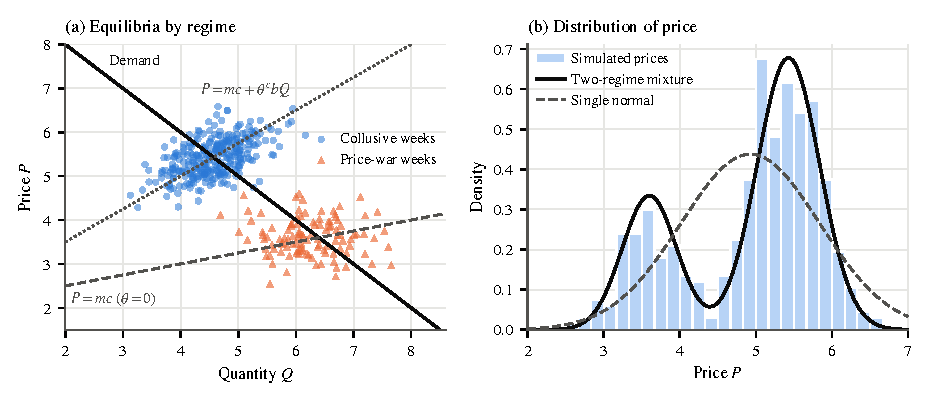
\includegraphics[width=\textwidth]{figures/ch01/regime_mixture.pdf}
\caption{Identification of conduct regimes from the distribution of the data. The simulated market has inverse demand
$P = 10 - Q + u^d$ and marginal cost $mc = 2 + 0.25\,Q + u^c$, observed for 400 weeks. Conduct is collusive
($\theta^{c} = 0.5$) with probability $\varpi = 0.7$ and competitive ($\theta^{w} = 0$) otherwise, with
$u^d \sim N(0, 0.8^2)$ and $u^c \sim N(0, 0.4^2)$. Panel (a) colors each week by its true regime, which the analyst does not observe, and draws the deterministic demand
curve and the two supply relations. Panel (b) shows the distribution of price that the analyst sees. The two-regime
mixture fits it, while a single normal distribution does not. The regime means of price, $3.6$ and $5.43$, differ by
more than four within-regime standard deviations, so the distribution is bimodal. Closer regimes could produce a single
mode. All values are illustrative.}
\label{fig:01-regimes}
\end{figure}

The main threat to this inference is that some other unobserved shock moves the supply relation. Because the
identifying variation is an error component, nothing in the procedure guarantees the conduct interpretation. Unrecorded
changes in factor prices or technology could produce the same pattern, and Porter had no factor-price data. Bresnahan
finds the conduct interpretation likely in the railroad case for two reasons. The regime shifts move price and quantity
by about 50 percent, and contemporary sources discuss cartel adherence extensively. An alternative is to fix the sample
split in advance and estimate $\theta^{c}$ and $\theta^{w}$ separately, as \citet{Bresnahan1987} does. This needs prior
information but allows a more direct check that the apparent supply shocks reflect conduct. \Cref{ch:collusion-evidence}
returns to these issues with \citet{Porter1983} and \citet{Ellison1994}.

\subsubsection{Comparative statics in industry structure}\label{sec:01-id-structure}

The fifth argument relates price to the number of firms or to concentration across similar local markets. Its logic is
familiar, but \citet[p.~1032]{Bresnahan1989} judges that it still awaited its identification arguments.
\Cref{sec:01-price-concentration} presented these studies and the six difficulties Bresnahan raises. In the language of
this section, all of them come back to the aggregate supply relation \eqref{eq:01-avg-supply}, which is
\cref{prop:01-supply-relation}(ii) applied market by market. A lower price in markets with more firms can mean lower
average conduct $\theta$ or lower average marginal cost $\overline{mc}$. Price and quantity data alone cannot apportion
the change between the two. A change in entry regulation, as in \citet{SpillerFavaro1984}, offers cleaner
variation because it moves structure for a reason unrelated to costs. The arguments of this section can then separate
the two channels, for example by checking whether demand rotations identify a lower $\theta$ after deregulation.

\subsubsection{Synthesis}\label{sec:01-id-synthesis}

\Cref{tab:01-id-strategies} summarizes the arguments. Their variety reflects the variety of data across industry
studies \citep[Section~3.6]{Bresnahan1989}. Each industry offers different information and institutional detail, and
therefore different defenses of different methods. The variety also reflects how many comparative statics of markets
with market power have no counterpart in competitive markets.

\begin{table}[htbp]
\centering
\begin{threeparttable}
\caption{How the data identify market power}
\label{tab:01-id-strategies}
\footnotesize
\setlength{\tabcolsep}{4pt}
\begin{tabularx}{\textwidth}{@{}>{\raggedright\arraybackslash}p{2.05cm}
  >{\raggedright\arraybackslash}X >{\raggedright\arraybackslash}X >{\raggedright\arraybackslash}X
  >{\raggedright\arraybackslash}p{2.2cm} >{\raggedright\arraybackslash}p{1.8cm}@{}}
\toprule
Argument & Exogenous variation & What is identified & Key maintained assumption & Applications & Full treatment \\
\midrule
Comparative statics in demand & Demand shifters that rotate demand ($Y_t$ entering $P_Q$) & Conduct $\theta$ and
  the slope of marginal cost separately & Correct demand specification; demand not of the form $\tilde P(Q, h(Y))$ &
  \citet{JustChern1980}; \citet{Bresnahan1981,Bresnahan1987} & \cref{ch:conduct} \\
\addlinespace
Homogeneity of marginal cost & Factor prices & $\theta$ from terms not multiplied by factor prices & Marginal cost
  homogeneous of degree one in observed factor prices & \citet{Appelbaum1979,Appelbaum1982} & \cref{ch:conduct} \\
\addlinespace
Comparative statics in cost & All factor prices, or taxes & Sign of $\psi$; bound on $\sum_i (1 + r_i)^{-1}$ &
  All cost shifters measured; long-run equilibrium (for $\psi$); known link to marginal cost &
  \citet{PanzarRosse1977}; \citet{Shaffer1982}; \citet{Sullivan1985}; \citet{AshenfelterSullivan1987} &
  \cref{ch:conduct} \\
\addlinespace
Direct estimation of marginal cost & Factor prices with input quantities & Marginal cost from factor demands, then
  $\theta$ & Cost-function form; correct price of capital services & \citet{GollopRoberts1979};
  \citet{Appelbaum1982}; \citet{Hall1988} & \cref{sec:01-rising-markups} \\
\addlinespace
Supply shocks & Unobserved two-valued shock to the supply relation & Frequency and size of regime changes in conduct &
  No other unobserved shifts in the supply relation & \citet{Porter1983}; \citet{LeePorter1984} &
  \cref{ch:collusion-evidence} \\
\addlinespace
Comparative statics in structure & Number of firms or concentration across local markets & Reduced-form price and
  structure relation & Structure exogenous; average cost unrelated to structure & \citet{GrahamKaplanSibley1983};
  \citet{SpillerFavaro1984} & \cref{sec:01-price-concentration} \\
\addlinespace
Residual demand & Cost shifters specific to one firm & Elasticity of the firm's residual demand & Firm's costs move
  independently of rivals' costs & \citet{BakerBresnahan1988} & \cref{ch:conduct} \\
\bottomrule
\end{tabularx}
\begin{tablenotes}\footnotesize
\item Notes: The first six rows follow the classification of \citet[Section~3]{Bresnahan1989} and are introduced in
\cref{sec:01-id-arguments}. The last row is the summary-statistic approach of his Section~4, introduced in
\cref{sec:01-neio-diffprod}. The last column gives the place in this book where each argument is developed in full.
\end{tablenotes}
\end{threeparttable}
\end{table}

\subsection{Market power with product differentiation}\label{sec:01-neio-diffprod}

Product differentiation raises short-run and long-run questions \citep[Section~4]{Bresnahan1989}. In the short run the
set of products and their attributes are fixed, and we ask how much market power existing differentiation confers. The
question has two parts. As products become more distinct, each firm's profit depends less on rivals' prices, which the
own- and cross-price elasticities of demand measure. As products become more distinct, each firm also responds less to
rivals' moves, which requires a model of competitive interaction.

The conceptual issues resemble those of the homogeneous-good case, but measurement is much harder. Suppose an industry
has $J$ products and we assume constant elasticities and symmetric cross effects. Demand still has $J$ own-price
elasticities, $J$ income elasticities and $\frac{J(J - 1)}{2}$ cross-price elasticities. With $J = 100$ products this is
\begin{equation*}
J + J + \frac{J(J - 1)}{2} = 100 + 100 + 4{,}950 = 5{,}150
\end{equation*}
elasticities, and few industries have fewer than 100 products. Multi-product firms may also have economies of scope.
Prior information from trade journals and marketing studies becomes indispensable, and how it is used varies from
industry to industry.

The most common shortcut treats the products as close substitutes, uses a price index as the observed price, and
proceeds as for a homogeneous good. Bresnahan warns that this can attribute to conduct what is due to product
differentiation \citep[p.~1046]{Bresnahan1989}. The next example makes the warning precise.

\begin{example}[Differentiation that looks like conduct]\label{ex:01-index-conduct}
Let $J$ symmetric single-product firms set prices in a Bertrand equilibrium with constant marginal cost. Let
$\varepsilon_{\mathrm{own}} > 0$ be each product's own-price elasticity (as a positive number) and
$\varepsilon_{\mathrm{cross}} \ge 0$ the cross-price elasticity between any two products. The pricing rule of
\cref{prop:01-pricing-rule} gives each firm the Lerner index $L = \frac{1}{\varepsilon_{\mathrm{own}}}$. An analyst
who treats the products as one homogeneous good measures the market elasticity when all prices move together,
\begin{equation*}
\varepsilon = \varepsilon_{\mathrm{own}} - (J - 1)\,\varepsilon_{\mathrm{cross}} ,
\end{equation*}
and reads conduct from $\frac{P - mc}{P} = \frac{\theta}{\varepsilon}$. The apparent conduct parameter is
\begin{equation*}
\tilde\theta = \varepsilon L = \frac{\varepsilon_{\mathrm{own}} - (J - 1)\,\varepsilon_{\mathrm{cross}}}{\varepsilon_{\mathrm{own}}}
 = 1 - (J - 1)\,D, \qquad D = \frac{\varepsilon_{\mathrm{cross}}}{\varepsilon_{\mathrm{own}}} .
\end{equation*}
With symmetric quantities, $D$ is the \emph{diversion ratio} between two products, the fraction of the sales lost by one
product that go to another when its price rises (\cref{ch:diffprod}). So $\tilde\theta$ is the fraction of lost sales that leave
the industry. It lies between zero and one although no firm colludes. With $J = 4$, $\varepsilon_{\mathrm{own}} = 4$ and
$\varepsilon_{\mathrm{cross}} = 1$ we get $\varepsilon = 1$, $L = 0.25$ and $\tilde\theta = 0.25$. This is exactly the
value of symmetric Cournot with four firms, produced by differentiated Bertrand competition.
\end{example}

To study differentiation directly, the analyst must reduce the dimension of the problem. Bresnahan describes three ways.

\casehead{Modeling product choice}
The first models how consumers choose among products, which yields demand systems with few parameters. Discrete-choice
models \citep[see][]{McFadden1984}, such as the nested logit, fit industries in which trade sources describe distinct
segments with much closer competition inside than across them. Spatial models of differentiation fit industries without
clear segment boundaries. In such industries, products A and B can both matter for C without A mattering for B. Spatial
models reduce the parameter count by localizing competition, and discrete-choice models do it by grouping. A
multinomial logit without nests is the limiting case in which the whole industry is one segment and competition is
symmetric. Bresnahan's spatial model of automobiles is an example \citep{Bresnahan1981,Bresnahan1987}. Any such model
is only as convincing as the information used to specify it, and the localized-versus-segmented distinction matters most.
\citet{Schmalensee1985b} proposes a test of localization based on how the prices and quantities of brands move together.
In ready-to-eat breakfast cereals he decisively rejects the model in which all brands compete equally, although he doubts
the covariance restrictions that identify the pattern of localization. \Cref{ch:discrete,ch:logit,ch:blp} develop the
modern versions of this approach.

\casehead{Aggregating products}
The second approach aggregates similar products until only a few elasticities remain. \citet{GelfandSpiller1987}
aggregate many types of bank loans into two and estimate a two-by-two system. Their model lets each bank's profit in
one market depend on rivals' strategies in both, an interdependence they write in conjectural-variations form.
\citet{Slade1987} studies ``majors'' and ``independents'' among gasoline stations in Vancouver. \citet{Suslow1986}
aggregates output into the dominant firm's product and the fringe's product. The dominant firm's marginal revenue then
depends on the substitutability of the two products, the market elasticity and the fringe supply elasticity.

\casehead{Estimating a summary statistic: residual demand}
The third approach, due to \citet{BakerBresnahan1985,BakerBresnahan1988}, estimates only the summary statistic that
measures one firm's market power. Consider the seller of product 1, facing the inverse demand
\begin{equation}\label{eq:01-bb-demand}
P_1 = P^1(Q_1, P_2, \dots, P_J, Y, \gamma),
\end{equation}
where $P_2, \dots, P_J$ are the prices of competing products. The parameter vector $\gamma$ contains the cross effects of
all $J - 1$ rivals, so it can be very long. Each rival product $j = 2, \dots, J$ has its own demand equation like
\eqref{eq:01-bb-demand} and a supply relation
\begin{equation}\label{eq:01-bb-rival}
P_j = C_q^{j}(Q_j, W_j, Z_j, \Gamma_j) - \frac{\partial P^{j}}{\partial Q_j}\, Q_j\, \vartheta_j ,
\qquad j = 2, \dots, J .
\end{equation}
These $2(J - 1)$ equations can be solved for the rivals' prices and quantities as functions of $Q_1$ and the exogenous
variables, $P_j = P_j^*(Q_1, W_{-1}, Z_{-1}, \Gamma_{-1}, \vartheta_{-1}, Y, \gamma)$. Here $W_{-1}$ and $Z_{-1}$ are the
rivals' cost shifters, and $Q_1$ remains because only the rivals' equations have been solved. Substituting into
\eqref{eq:01-bb-demand} gives the \emph{residual demand curve} of product 1,
\begin{equation}\label{eq:01-bb-residual}
P_1 = P^1\bigl(Q_1, P_2^*(\cdot), \dots, P_J^*(\cdot), Y, \gamma\bigr)
    \equiv P^{R}(Q_1, W_{-1}, Z_{-1}, \Gamma_{-1}, \vartheta_{-1}, Y, \gamma).
\end{equation}
Equations \eqref{eq:01-bb-demand} to \eqref{eq:01-bb-residual} are Bresnahan's (31), (4$^d$) and (32). By the chain rule,
the elasticity of residual inverse demand is
\begin{equation*}
-\frac{1}{\varepsilon^{R}_1} = \frac{\partial \ln P^{R}}{\partial \ln Q_1}
 = \frac{\partial \ln P^1}{\partial \ln Q_1} + \sum_{j = 2}^{J}\frac{\partial \ln P^1}{\partial \ln P_j}\,
   \frac{\partial \ln P_j^*}{\partial \ln Q_1} .
\end{equation*}
The first term is the direct effect of firm 1's output on its price. The sum adds the effect of rivals' price responses.
Substituting out the rivals' prices loses a great deal of information, since the separate elements of $\gamma$ can no
longer be estimated. That loss matters little for the question at hand. The slope of $P^{R}$ tells us how much power
firm 1 has over its price after all rivals have adjusted. Suppose product 1 is a perfect substitute for rival products
sold by price takers at constant cost. Then $P^{R}$ equals the lowest rival cost and does not respond to $Q_1$, so
$\frac{1}{\varepsilon^{R}_1} = 0$.

Residual demand can be estimated only if firm 1's costs move independently of its rivals' costs
\citep[fn.~43]{Bresnahan1989}. Its own cost shifters then serve as instruments for $Q_1$, while the rivals' cost
shifters enter \eqref{eq:01-bb-residual} directly. International markets offer natural experiments, since exchange-rate
movements change the relative costs of producers in different countries. The reciprocal
$\frac{1}{\varepsilon^{R}_1}$ of the residual-demand elasticity summarizes a firm's market power, but it does not reveal the sources of that power. It
equals the Lerner index only under particular conduct, for example when firm 1 acts as a Stackelberg leader toward
its rivals \citep[p.~289]{BakerBresnahan1988}. This is why Bresnahan leaves residual-demand studies out of his summary
table. The approach complements the
aggregation approach, which estimates every elasticity but only for a few products. \Cref{ch:conduct} treats
\citet{BakerBresnahan1988} and its application to brewing in depth.

\casehead{Market definition and policy}
These techniques bear on market definition in antitrust. Antitrust often asks whether a single firm has market power,
or whether a group of firms would have it if they acted together. \Cref{sec:01-market-definition} quoted Bresnahan's
remark that these questions are well posed even where computing shares in a relevant market is senseless. Residual
demand answers the first question directly. \citet{ScheffmanSpiller1987} extend
it to a group of firms, which answers the second. \citet{BakerBresnahan1985} ask how much steeper the residual demand of
two merging firms would be after the merger. If the two sell close substitutes and few other firms sell similar products,
each firm is an important brake on the other, and the merger steepens the curve. The Panzar-Rosse statistic gives a
related answer. A rejection of monopoly for a firm or group means that it cannot be treated as acting in isolation.
\Cref{ch:mergers} develops merger analysis with differentiated products.

\casehead{Differentiation in the long run}
In the long run firms add products, change attributes or perceptions, and new firms enter with new products or
imitations. Theory offers many strategic hypotheses: preemption by reputation for quality, preemption by filling the
product space, and coordination of product choices to soften competition. In 1989 essentially nothing empirical was known
about any of them \citep[p.~1050]{Bresnahan1989}. The same passage contains the welfare point of
\cref{sec:01-fixed-costs}. Under the Chamberlin tangency every firm prices above marginal cost, so short-run market power
says little about efficiency until we know how new products and new firms are supplied.

\subsection{What the NEIO learned}\label{sec:01-neio-lessons}

The case-study character of the NEIO raises questions of interpretation \citep[Section~5]{Bresnahan1989}. How general
are the results, and what do they reveal about market power in the economy as a whole? The SCP paradigm aimed to estimate
a map from structure to conduct and performance. Such a map would be valuable, for example to guide merger policy, which
acts on structure. A single industry study reveals at most one point on it. By 1989 NEIO studies covered more than a
dozen industries. \Cref{tab:01-bresnahan-table} reproduces the estimated Lerner indices that Bresnahan collected.

\begin{table}[htbp]
\centering
\begin{threeparttable}
\caption{Estimated Lerner indices from early NEIO studies}
\label{tab:01-bresnahan-table}
\small
\begin{tabular}{@{}llc@{}}
\toprule
Author & Industry & $L$ \\
\midrule
\citet{Lopez1984} & Food processing & 0.504 \\
\citet{Roberts1984} & Coffee roasting & 0.055 / 0.025$^{a}$ \\
\citet{Appelbaum1982} & Rubber & 0.049$^{c}$ \\
\citet{Appelbaum1982} & Textile & 0.072$^{c}$ \\
\citet{Appelbaum1982} & Electrical machinery & 0.198$^{c}$ \\
\citet{Appelbaum1982} & Tobacco & 0.648$^{c}$ \\
\citet{Porter1983} & Railroads & 0.40$^{b}$ \\
\citet{Slade1987} & Retail gasoline & 0.10 \\
\citet{Bresnahan1981} & Automobiles (1970s) & 0.1 / 0.34$^{d}$ \\
\citet{Suslow1986} & Aluminum (interwar) & 0.59 \\
\citet{SpillerFavaro1984} & Banks ``before''$^{e}$ & 0.88 / 0.21$^{f}$ \\
\citet{SpillerFavaro1984} & Banks ``after''$^{e}$ & 0.40 / 0.16$^{f}$ \\
\bottomrule
\end{tabular}
\begin{tablenotes}\footnotesize
\item Notes: $L = \frac{P - mc}{P}$. $^{a}$Largest and second-largest firm, respectively. $^{b}$When the cartel was
succeeding (0 in reversionary periods). $^{c}$At the sample midpoint. $^{d}$Varies by type of car, larger in the standard
and luxury segments. $^{e}$Uruguayan banks before and after entry deregulation. $^{f}$Large firms / small firms.
Panzar-Rosse and Sullivan studies are excluded because they yield only tests of, or bounds on, conduct.
Residual-demand studies are excluded because the reciprocal $\frac{1}{\varepsilon^{R}}$ of the residual-demand elasticity
equals the Lerner index only in special cases.
\item Source: \citet{Bresnahan1989}, Table~17.1.
\end{tablenotes}
\end{threeparttable}
\end{table}

From this evidence Bresnahan draws three guarded conclusions \citep[pp.~1052--1053]{Bresnahan1989}.

\casehead{Conclusion A}
Some concentrated industries have a great deal of market power, in the sense of high price-cost margins. Several entries
in \cref{tab:01-bresnahan-table} exceed 0.4. The industries cannot be matched systematically to census concentration
measures, because many data sets were collected by the authors. A glance at the list shows that they come overwhelmingly
from the concentrated end of the spectrum.

Two reasons warn against generalizing. First, researchers who invent a method for detecting market power apply it first
where they expect to find it. They choose concentrated industries, known or suspected cartels, or industries where earlier
case studies suggested anticompetitive conduct. Second, the data often come from trade journals, regulators or court records.
Industries with excellent trade journals are industries in which firms know a lot about their rivals, an information
structure that favors collusion. Suslow could use the trial record on Alcoa because Alcoa was suspected of market power.
More sources of data, from more industries, were needed.

\casehead{Conclusion B}
One significant cause of high margins is anticompetitive conduct. The studies separate conduct, the behavioral rules by
which firms set prices, from performance, the price-cost margin. They do not find small departures from price taking
combined with very steep demand. Several find conduct well toward the collusive end. \citet{Porter1983} and \citet{Bresnahan1987}
both find collusive conduct, although of different kinds. The railroads in Porter's study had formed the JEC by a
publicly acknowledged agreement \citep[p.~302]{Porter1983}. \citet[pp.~457 and 479]{Bresnahan1987} interprets automobile
pricing in 1954 and 1956 as tacit collusion, meaning collusive pricing without an explicit agreement among firms. His
tests compare a collusive pricing model with a Bertrand model, so they cannot reveal whether the automakers
communicated. Conduct is not uniform. \citet{Roberts1984} classifies most
coffee roasters as a price-taking fringe, while the largest firms behave less competitively without reaching the profit
maximum given the fringe.

\casehead{Conclusion C}
The new methods had taught little about the relation between market power and industry structure. The studies cover only
the concentrated end of the range, so they reveal the structure-performance map over a narrow interval. Few of them
address the causes of market power. Long-lived market power suggests that entry fails to discipline conduct, yet the
studies hardly discuss entry.

\casehead{The sources of market power}
Bresnahan closes by pointing to the causes of market power as the frontier \citep[Section~6]{Bresnahan1989}. Entry,
predation, entry deterrence and long-run strategic competition had received little empirical work with explicit
theoretical foundations. \citet{Burns1986} studies the American tobacco trust and finds that its acquisitions of
competitors became cheaper after episodes of predatory pricing. The study relies on a nineteenth-century documentary record
that modern firms would not leave. The open problem was to find the empirical implications of predation when predatory acts
must be inferred. On entry, \citet{PanzarRosse1977} add to demand and the supply relations an entry condition for the
marginal firm, $P = \mathit{LRAC}(W, Y)$, with $\mathit{LRAC}$ long-run average cost.
\citet{BresnahanReiss1990} model the entry decisions of the first two firms in a market with an integer number of firms.
They use 149 geographically isolated American markets for new car dealers. A second entrant faces nearly the same costs
and opportunities as the first, and its entry does not lower the monopoly dealer's margins by much. Both papers
argue that cross-sections of closely related markets are the right samples for studying entry. \Cref{sec:01-today-structure}
takes up the sequel by \citet{BresnahanReiss1991}.

Bresnahan's final assessment is optimistic about measurement and modest about explanation. By abandoning accounting
measures of performance, the NEIO produced a new kind of evidence of substantial market power, immune to the standard
criticisms of earlier work. Its studies are detailed enough that alternative explanations can be confronted and rebutted.
In his words, ``we know that there is market power out there, and need to know a lot more about exactly where''
\citep[p.~1055]{Bresnahan1989}. Its causes and systematic predictors remained essentially unknown.

The program that followed kept the NEIO's commitment to single industries and explicit models. Its main change was on the
demand side. Classic analyses of market power, such as \citet{Porter1983}, \citet{Bresnahan1987} and
\citet{Nevo2001}, supply the basic toolkit \citep[p.~151]{EinavLevin2010}. That toolkit combines demand and supply in
an equilibrium analysis of imperfect competition. Modern work replaces the conduct parameter with explicit models of differentiated-product
competition and estimates rich demand systems with instruments. \Cref{sec:01-today} describes this structural workflow.
